%%%%%%%%%%%%%%%%%%%%%%%%%%%%%%%%%%%%%%%%%%%%%%%%%%%%%%%%%%%%%%
% CHAPTER 7
%%%%%%%%%%%%%%%%%%%%%%%%%%%%%%%%%%%%%%%%%%%%%%%%%%%%%%%%%%%%%%

\chapter{Experimentation and Model Development}
\label{chap:experimentation_model_development}

\markboth{Chapter 7}{Experimentation and Model Development}

%%%%%%%%%%%%%%%%%%%%%%%%%%%%%%%%%%%%%%%%%%%%%%%%%%%%%%%%%%%%%%
\section{Introduction}

This chapter presents the experimentation and model-development
process carried out for the proposed
\textbf{DocSaarthi: AI Legal \& Financial Document Assistant}.
The objective of the experimentation stage was to evaluate different
processing strategies for document classification, information
retrieval, bilingual interaction, translation, and
source-grounded question answering.

The experiments were designed according to the implemented prototype
described in the previous chapter. Since the current implementation
does not perform large-scale transformer fine-tuning, the experiments
focus on lexical and rule-based processing, document chunk matching,
intent routing, translation, and optional AI-based answer generation.

The experimentation process was used to identify a practical
configuration that provides reliable document-based responses while
preserving important legal and financial information such as dates,
monetary values, percentages, clauses, and page references.

%%%%%%%%%%%%%%%%%%%%%%%%%%%%%%%%%%%%%%%%%%%%%%%%%%%%%%%%%%%%%%
\section{Experimental Design}

The experimental design was divided into multiple stages to evaluate
the individual components of the DocSaarthi pipeline.

The major experimental stages were:

\begin{enumerate}
    \item Preparation and inspection of the 400-record Hindi intent
    dataset.
    \item Testing of PDF text extraction and page-level text
    preservation.
    \item Evaluation of text preprocessing and document chunking.
    \item Testing of lexical query-to-document matching.
    \item Evaluation of Legal and Financial document classification.
    \item Testing of English--Hindi translation.
    \item Evaluation of source-grounded question answering.
    \item Comparison of local answer generation with optional
    AI-assisted answer generation.
    \item Evaluation of page-level evidence and unsupported-question
    handling.
\end{enumerate}

The experimental workflow is summarized below.

\begin{figure}[H]
    \centering
    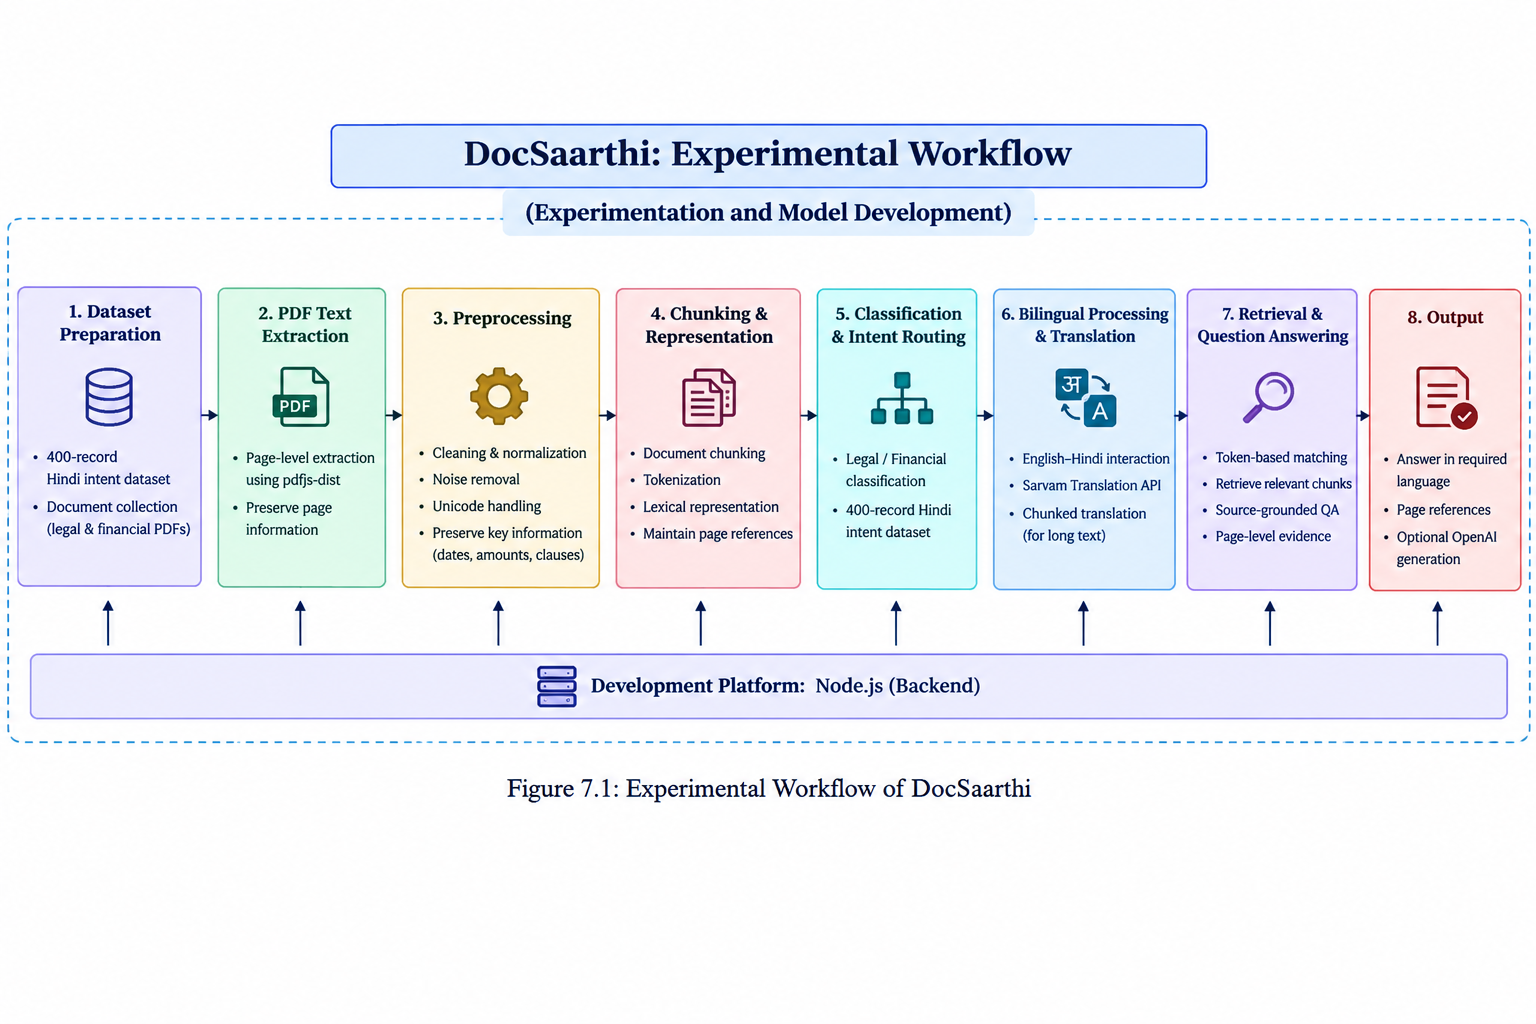
\includegraphics[width=0.95\textwidth]{figures/experimental_workflow.png}
    \caption{Experimental Workflow of DocSaarthi}
    \label{fig:experimental_workflow}
\end{figure}

The same document set was used wherever possible so that different
processing configurations could be compared under similar
conditions.

%%%%%%%%%%%%%%%%%%%%%%%%%%%%%%%%%%%%%%%%%%%%%%%%%%%%%%%%%%%%%%
\section{Baseline Model}

A baseline configuration was established to provide a reference for
evaluating the proposed document-intelligence pipeline.

The baseline approach uses direct document text processing with
basic lexical matching and limited preprocessing. User queries are
matched against the extracted document text without applying the
complete bilingual retrieval and evidence-handling workflow.

The baseline configuration consists of:

\begin{itemize}
    \item Basic PDF text extraction.
    \item Basic text cleaning.
    \item Direct keyword-based matching.
    \item Simple document category identification.
    \item Direct response generation from matched text.
\end{itemize}

The baseline provides a simple reference implementation against which
the improvements introduced by the proposed configuration can be
observed.

\begin{table}[H]
\centering
\caption{Baseline Configuration}
\begin{tabular}{|p{5cm}|p{8cm}|}
\hline
\textbf{Component} & \textbf{Baseline Configuration} \\
\hline
PDF Processing & Basic page-level text extraction \\
\hline
Preprocessing & Basic cleaning and whitespace handling \\
\hline
Representation & Keyword/token representation \\
\hline
Retrieval & Direct lexical matching \\
\hline
Classification & Basic content-based classification \\
\hline
Translation & External translation service when required \\
\hline
Question Answering & Direct response from matched content \\
\hline
Evidence & Limited page-level reference handling \\
\hline
\end{tabular}
\end{table}

The baseline experiment was useful for identifying the limitations of
simple keyword matching, especially for long documents and
cross-language questions.

%%%%%%%%%%%%%%%%%%%%%%%%%%%%%%%%%%%%%%%%%%%%%%%%%%%%%%%%%%%%%%
\section{Proposed Model}

The proposed configuration extends the baseline approach by
introducing a modular source-grounded document-processing pipeline.

The proposed system combines preprocessing, document chunking,
lexical retrieval, bilingual interaction, structured information
extraction, translation, and evidence-based question answering.

The major components of the proposed configuration are:

\begin{enumerate}
    \item PDF upload and validation.
    \item Page-level PDF text extraction.
    \item Unicode normalization and text cleaning.
    \item Document chunking.
    \item Legal/Financial document classification.
    \item Structured information extraction.
    \item Hindi intent routing using the 400-record dataset.
    \item Bilingual query processing.
    \item Token-based document retrieval.
    \item English--Hindi translation using the Sarvam API.
    \item Source-grounded question answering.
    \item Page-level evidence presentation.
    \item Optional OpenAI-based answer generation.
\end{enumerate}

The proposed configuration maintains the original document as the
authoritative source of information. The intent dataset is used for
question routing and is not treated as evidence for document answers.

\begin{table}[H]
\centering
\caption{Proposed Model Configuration}
\begin{tabular}{|p{5cm}|p{8cm}|}
\hline
\textbf{Component} & \textbf{Proposed Configuration} \\
\hline
PDF Processing & Page-level extraction using \texttt{pdfjs-dist} \\
\hline
Preprocessing & Cleaning, Unicode normalization and chunking \\
\hline
Representation & Normalized tokens and document chunks \\
\hline
Classification & Lexical/heuristic Legal-Financial classification \\
\hline
Intent Routing & 400-record Hindi intent dataset \\
\hline
Retrieval & Token and lexical document matching \\
\hline
Translation & Sarvam Translation API \\
\hline
Question Answering & Source-grounded document QA \\
\hline
Answer Enhancement & Optional OpenAI-based generation \\
\hline
Evidence & Page-level document references \\
\hline
Fallback & ``Not found'' response for insufficient evidence \\
\hline
\end{tabular}
\end{table}

%%%%%%%%%%%%%%%%%%%%%%%%%%%%%%%%%%%%%%%%%%%%%%%%%%%%%%%%%%%%%%
\section{Feature Representation Experiments}

Feature representation experiments were conducted to determine how
document and query text should be represented for effective matching.

Since the current prototype does not train a new transformer model,
the experiments focused on lexical and structured representations.

\subsection{Raw Text Representation}

In the initial experiment, extracted document text was retained as
plain text. This representation was useful for preserving the original
content but was less effective for direct matching in long documents.

Long documents contained formatting inconsistencies, repeated
whitespace, and line breaks that could reduce the effectiveness of
simple matching.

\subsection{Normalized Token Representation}

The next experiment applied text normalization and tokenization.
Important terms were converted into a consistent representation before
matching.

This representation improved the ability to identify relevant
document sections when the query and document used similar terminology.

\subsection{Chunk-Based Representation}

The document was divided into smaller searchable chunks while
retaining the original page reference.

Chunk-based representation improved retrieval because the system could
identify smaller portions of a document rather than processing the
complete document for every question.

\subsection{Structured Information Representation}

Structured information such as dates, monetary values, percentages,
clauses, and document classification was maintained separately from
the general text representation.

This representation is particularly useful for legal and financial
questions where numerical and contractual information must be
preserved accurately.

\begin{table}[H]
\centering
\caption{Feature Representation Experiments}
\begin{tabular}{|p{4cm}|p{5cm}|p{4cm}|}
\hline
\textbf{Representation} & \textbf{Purpose} & \textbf{Observation} \\
\hline
Raw Text & Preserve extracted document content & Simple but less suitable for long-document matching \\
\hline
Normalized Tokens & Improve lexical matching & More consistent query matching \\
\hline
Document Chunks & Retrieve relevant sections & Improved focused retrieval and evidence tracking \\
\hline
Structured Values & Preserve dates and numerical information & Useful for legal and financial queries \\
\hline
\end{tabular}
\end{table}

%%%%%%%%%%%%%%%%%%%%%%%%%%%%%%%%%%%%%%%%%%%%%%%%%%%%%%%%%%%%%%
\section{Model Comparison}

The baseline and proposed configurations were compared using
functional and qualitative criteria relevant to the DocSaarthi
application.

The comparison focused on retrieval quality, bilingual support,
document verification, handling of long documents, and resistance to
unsupported answers.

\begin{table}[H]
\centering
\caption{Baseline and Proposed Model Comparison}
\begin{tabular}{|p{5cm}|p{3.5cm}|p{3.5cm}|}
\hline
\textbf{Parameter} & \textbf{Baseline} & \textbf{Proposed} \\
\hline
Text Preprocessing & Basic & Normalization and cleaning \\
\hline
Document Chunking & Limited & Implemented \\
\hline
Query Matching & Direct lexical matching & Chunk and token-based matching \\
\hline
Bilingual Interaction & Limited & English--Hindi support \\
\hline
Intent Routing & Not emphasized & 400-record Hindi intent dataset \\
\hline
Information Extraction & Basic & Structured extraction \\
\hline
Translation & External translation when required & Integrated translation layer \\
\hline
Evidence Tracking & Limited & Page-level evidence \\
\hline
Unsupported Questions & May produce weak matches & ``Not found'' fallback \\
\hline
Answer Generation & Direct response & Grounded response with optional AI enhancement \\
\hline
\end{tabular}
\end{table}

The proposed configuration provides a more complete workflow for
document understanding because retrieval, translation, evidence
tracking, and answer generation are integrated into the same pipeline.

%%%%%%%%%%%%%%%%%%%%%%%%%%%%%%%%%%%%%%%%%%%%%%%%%%%%%%%%%%%%%%
\section{Hyperparameter Experimentation}

The current prototype does not perform neural network training or
transformer fine-tuning. Therefore, conventional training
hyperparameters such as learning rate, batch size, and number of
epochs are not applicable to the implemented system.

Instead, experimentation was performed on processing parameters that
affect document retrieval and response generation.

The important configurable parameters include:

\begin{itemize}
    \item Document chunk size.
    \item Amount of text overlap between chunks.
    \item Number of retrieved document chunks.
    \item Lexical matching threshold.
    \item Maximum translation text length.
    \item Query normalization rules.
    \item Answer-generation configuration.
\end{itemize}

These parameters were adjusted to achieve a balance between retrieval
coverage, response relevance, processing time, and API limitations.

\begin{table}[H]
\centering
\caption{Processing Parameter Experimentation}
\begin{tabular}{|p{5cm}|p{4cm}|p{4cm}|}
\hline
\textbf{Parameter} & \textbf{Effect of Increasing Value} & \textbf{Experimental Consideration} \\
\hline
Chunk Size & More context per retrieval unit & Very large chunks may reduce retrieval precision \\
\hline
Chunk Overlap & Better continuity between sections & Excessive overlap increases repeated content \\
\hline
Retrieved Chunks & More contextual information & Too many chunks may introduce irrelevant text \\
\hline
Matching Threshold & Stricter relevance filtering & Excessive threshold may miss valid evidence \\
\hline
Translation Chunk Length & Larger translation context & Very large inputs may exceed service limits \\
\hline
\end{tabular}
\end{table}

The final processing configuration was selected based on practical
testing with the implemented document-processing workflow.

%%%%%%%%%%%%%%%%%%%%%%%%%%%%%%%%%%%%%%%%%%%%%%%%%%%%%%%%%%%%%%
\section{Experimental Observations}

The experiments produced several important observations.

\subsection{Observation 1: Importance of Preprocessing}

Raw PDF text cannot always be used directly for reliable retrieval.
Line breaks, repeated spaces, and formatting inconsistencies can
affect lexical matching. Text normalization therefore improves the
consistency of the document representation.

\subsection{Observation 2: Importance of Chunking}

Chunking improves retrieval for long legal and financial documents.
Instead of searching the entire document as a single unit, the system
can identify smaller sections that are more closely related to the
user's question.

\subsection{Observation 3: Importance of Page References}

Maintaining page information during extraction and chunking is
important for document verification. Users can trace the generated
response back to the relevant section of the original document.

\subsection{Observation 4: Bilingual Interaction}

Translation enables users to interact with English documents using
Hindi questions and responses. However, translation is maintained as
a separate processing layer so that the original English document
remains unchanged.

\subsection{Observation 5: Source Grounding}

Restricting answers to retrieved document evidence reduces the risk of
providing information that is not present in the uploaded document.
When adequate evidence cannot be retrieved, the system can return a
``not found'' response.

\subsection{Observation 6: External Service Dependency}

The translation and optional AI answer-generation components depend on
external services. Therefore, error handling and fallback mechanisms
are required to maintain system usability when external services are
unavailable.

\subsection{Observation 7: Intent Dataset Usage}

The 400-record Hindi dataset is useful for identifying and routing
user query intents. However, it is not used as the authoritative
knowledge source for document answers.

%%%%%%%%%%%%%%%%%%%%%%%%%%%%%%%%%%%%%%%%%%%%%%%%%%%%%%%%%%%%%%
\section{Selected Model and Configuration}

Based on the experimentation, the proposed source-grounded
configuration was selected for the DocSaarthi prototype.

The selected configuration combines lexical document retrieval,
document chunking, structured information extraction, bilingual
translation, intent routing, and page-level evidence.

\begin{table}[H]
\centering
\caption{Selected Model and Configuration}
\begin{tabular}{|p{5cm}|p{8cm}|}
\hline
\textbf{Component} & \textbf{Selected Configuration} \\
\hline
Programming Language & JavaScript \\
\hline
Runtime & Node.js 20 or later \\
\hline
PDF Processing & \texttt{pdfjs-dist} \\
\hline
Text Representation & Normalized tokens and document chunks \\
\hline
Document Classification & Lexical/heuristic analysis \\
\hline
Intent Dataset & 400 labelled Hindi records \\
\hline
Retrieval & Token and lexical matching \\
\hline
Translation & Sarvam Translation API \\
\hline
Question Answering & Source-grounded document QA \\
\hline
AI Enhancement & Optional OpenAI answer generation \\
\hline
Evidence & Page-level references \\
\hline
Fine-tuning & Not performed \\
\hline
\end{tabular}
\end{table}

The selected configuration provides a practical balance between
implementation complexity, processing requirements, bilingual
functionality, and document-grounded response generation.

%%%%%%%%%%%%%%%%%%%%%%%%%%%%%%%%%%%%%%%%%%%%%%%%%%%%%%%%%%%%%%
\section{Stage 3 Readiness}

The experimentation stage prepares the DocSaarthi prototype for the
next stage of development and evaluation.

The following components are ready for further testing:

\begin{itemize}
    \item PDF upload and validation.
    \item Page-level PDF text extraction.
    \item Text preprocessing and normalization.
    \item Document chunking.
    \item Legal/Financial document classification.
    \item Structured information extraction.
    \item Hindi intent dataset integration.
    \item English--Hindi translation.
    \item Bilingual document retrieval.
    \item Source-grounded question answering.
    \item Page-level evidence presentation.
    \item Optional AI-based answer generation.
\end{itemize}

The next stage can focus on systematic evaluation of the implemented
system using representative legal and financial documents. Evaluation
can include retrieval relevance, classification correctness,
translation quality, answer correctness, evidence coverage, response
time, and handling of unsupported questions.

The system can also be extended in future experiments by introducing
trained multilingual models such as IndicBERT, MuRIL, or IndicTrans2
when sufficient computational resources and labelled training data
are available. Such models are not considered part of the current
implemented prototype.

%%%%%%%%%%%%%%%%%%%%%%%%%%%%%%%%%%%%%%%%%%%%%%%%%%%%%%%%%%%%%%
\section*{Chapter Summary}

This chapter presented the experimentation and model-development
process for the \textbf{DocSaarthi} system. The experimental design,
baseline configuration, proposed configuration, feature
representation experiments, model comparison, processing parameter
experimentation, and experimental observations were discussed.

The experiments showed the importance of preprocessing, document
chunking, lexical retrieval, bilingual interaction, structured
information extraction, and page-level evidence for building a
reliable legal and financial document assistant.

The source-grounded proposed configuration was selected as the final
prototype configuration. The system is now prepared for systematic
evaluation and further development in the next stage of the project.

%%%%%%%%%%%%%%%%%%%%%%%%%%%%%%%%%%%%%%%%%%%%%%%%%%%%%%%%%%%%%%